\newif\ifanswer\answertrue
%\answerfalse
\answerfalse

\documentclass[10pt,dvipdfmx]{jsarticle}
\usepackage[margin=15truemm]{geometry}
\usepackage[dvipdfmx]{graphicx}
\usepackage{wrapfig}
\usepackage[dvipdfmx]{color}
\usepackage{ascmac} % for scree
\usepackage{subfigure} % for subfigure
\usepackage{multicol}
\usepackage{setspace}
\usepackage{diagbox}
\usepackage{fancyhdr}
\usepackage{xcolor}
\usepackage{here}
\usepackage{amsmath}
\usepackage{amssymb}
\usepackage{tikz}
\usetikzlibrary{intersections, calc, arrows.meta}
\pagestyle{fancy}
\ifanswer
\lhead{数IA 解答}
\else
\lhead{数IA}
\fi
\rhead{\number\month\number\day}

\ifanswer
\newcommand{\answer}[2]{{\color{orange}#2}}
\newcommand{\page}[2]{#1}
\newcommand{\question}[2]{{\color{orange}#2}}
\else
\newcommand{\answer}[2]{\vspace{#1mm}}
\newcommand{\page}[2]{#2}
\newcommand{\question}[2]{#1}
\fi%answer

\begin{document}
\section*{I}
\subsection*{数と式}
\subsubsection*{展開}
\begin{Large}
  \begin{itemize}
    \item $(a+b+c)^2=$
    \item $(a+b)^3=$
    \item $(a-b)^3=$
    \item $(x+y)(x^2-xy+y^2)=$
    \item $(x-y)(x^2+xy+y^2)=$
  \end{itemize}
\end{Large}

\subsubsection*{因数分解}
\begin{Large}
  \begin{itemize}
    \item $a^2+b^2+c^2+2ab+2bc+2ca=$
    \item $x^3+3x^2y+3xy^2+y^3=$
    \item  $x^3-3x^2y+3xy^2-y^3=$
    \item $x^3+y^3=$
    \item $x^3-y^3=$
    \item $x^3+y^3+z^3-3xyz=$
  \end{itemize}
\end{Large}
\begin{itembox}[l]{因数分解の手順}
  \begin{Large}
    \begin{enumerate}
      \item %降べきの順
      \item %共通因数
      \item %公式
      \item %襷掛け
    \end{enumerate}
  \end{Large}
\end{itembox}

\begin{itembox}[l]{例題}
  \begin{large}
    \begin{enumerate}
      \item $3x^2+10x+3=$
      \item $x^2+xy-2y^2+4x+17y-21=$
      \item $a^2b+ab^2+b^2c+bc^2+c^2a+ca^2+2abc=$
    \end{enumerate}
  \end{large}
\end{itembox}

\subsubsection*{絶対値}
\begin{itembox}[l]{例題}
  \begin{large}
    \begin{enumerate}
      \item $|\pi-4|=$
      \item $|\sqrt{2}-1|+|\sqrt{2}-3|=$
    \end{enumerate}
  \end{large}
\end{itembox}
\subsection*{分母の有利化}
\begin{itembox}[l]{例題}
  \begin{large}
    \begin{enumerate}
      \item $\frac{1}{\sqrt{5}-\sqrt{3}}=$
    \end{enumerate}
  \end{large}
\end{itembox}
\subsubsection*{二重根号}
\begin{itembox}[l]{例題}
  \begin{large}
    \begin{enumerate}
      \item $\sqrt{6-\sqrt{20}}=$
      \item $\sqrt{14-4\sqrt{10}}=$
      \item $\sqrt{2+\sqrt{3}}=$
    \end{enumerate}
  \end{large}
\end{itembox}

\subsubsection*{対象式}
\begin{itembox}[l]{例題}
  $a=\frac{\sqrt{3}}{\sqrt{2}+1}, b=\frac{\sqrt{3}}{\sqrt{2}-1}$
  \begin{large}
    \begin{enumerate}
      \item $a+b$
      \item $ab$
      \item $a^2+b^2$
      \item $a^3+b^3$
    \end{enumerate}
  \end{large}
\end{itembox}



\subsubsection*{一次不等式}
\begin{itembox}[l]{ポイント}
  \vspace{8mm}

\end{itembox}
\begin{itembox}[l]{例題}
  \begin{large}
    \begin{enumerate}
      \item $x-5>3(7x-5)$
      \item $\frac{x+1}{2}\leqq\frac{2x+4}{3}$
      \item $=$
      \item $=$
    \end{enumerate}
  \end{large}
\end{itembox}

\subsubsection*{絶対値を含む等式・不等式}
\begin{itembox}[l]{例題}
  \begin{large}
    \begin{enumerate}
      \item $|5-x|=2$
      \item $|x-2|=2x-7$
      \item $|x-5|<3$
      \item $|x-5|\geqq3$
      \item $|2x-3|\geqq5x+1$
      \item $|x-2|+|x+1|=x+3$
    \end{enumerate}
  \end{large}
\end{itembox}

\newpage
\subsection*{二次関数}
\subsubsection*{一般式(2) グラフをかけ}
\begin{large}
  \begin{itemize}
    \item
    \item
  \end{itemize}
\end{large}

\begin{itembox}[l]{ポイント}
  \vspace{8mm}
\end{itembox}



\subsubsection*{最大最小}
\begin{itembox}[l]{場合分けの仕方(下に凸の場合)}
  \begin{itemize}
    \item 最小値\vspace{5cm}
    \item 最大値\vspace{5cm}
  \end{itemize}

\end{itembox}

\subsubsection*{解の個数の調べ方}
\begin{large}
  \begin{itemize}
    \item
  \end{itemize}
\end{large}

\subsubsection*{解の種類}
\begin{large}
  \begin{itemize}
    \item 二つの正の解
          \begin{itemize}
            \item \item \item
          \end{itemize}
    \item 二つの負の解
          \begin{itemize}
            \item \item \item
          \end{itemize}
    \item 正の解と負の解
          \begin{itemize}
            \item \item
          \end{itemize}
  \end{itemize}
\end{large}

\subsubsection*{二次不等式}
\begin{itembox}[l]{例題}
  \begin{large}
    \begin{multicols}{2}
      \begin{enumerate}
        \item $x^2-4x+3>0$
        \item $x^2-4x+3\leqq0$
        \item $x^2-4x+7\leqq0$
        \item $x^2-4x+4\geqq0$
        \item $x^2-4x+4>0$
        \item  $x^2-4x+4<0$
        \item $x^2-4x+4\leqq0$
      \end{enumerate}
    \end{multicols}
  \end{large}

\end{itembox}

\subsubsection*{解と係数の関係}
$ax^2+bx+c=0$の解を$\alpha,\beta$とする
\begin{multicols}{2}
  \begin{itemize}
    \item \item
  \end{itemize}
\end{multicols}


\newpage
\subsection*{図形}
\subsubsection*{定義}
\begin{minipage}[t]{0.5\textwidth}
  \begin{tikzpicture}
    \draw(0,0)--(4,0)--(4,3)--cycle;
  \end{tikzpicture}
\end{minipage}

\subsubsection*{代表角}
{\renewcommand\arraystretch{2}
  \begin{table}[H]
    \begin{tabular}{|c||p{1.5cm}|p{1.5cm}|p{1.5cm}|p{1.5cm}|p{1.5cm}|p{1.5cm}|p{1.5cm}|}
      \hline
      代表角 &  &  &  &  &  &  & \\
      \hline
      sin    &  &  &  &  &  &  & \\
      \hline
      cos    &  &  &  &  &  &  & \\
      \hline
      tan    &  &  &  &  &  &  & \\
      \hline
    \end{tabular}
  \end{table}
}

\subsubsection*{相互関係の公式}
\begin{LARGE}
  \begin{itemize}
    \item
    \item
    \item
  \end{itemize}
\end{LARGE}

\subsubsection*{正弦定理}
\begin{LARGE}
  \begin{itemize}
    \item
  \end{itemize}
\end{LARGE}
\subsubsection*{余弦定理}
\begin{LARGE}
  \begin{itemize}
    \item  \item  \item
  \end{itemize}
\end{LARGE}

\begin{itembox}[l]{正弦定理と余弦定理の使い分け}
  \vspace{8mm}
\end{itembox}


\subsubsection*{面積の求め方}
\begin{LARGE}
  \begin{itemize}
    \item  \item
  \end{itemize}
\end{LARGE}

\newpage
\subsection*{データ}
\subsubsection*{分散}
\begin{LARGE}
  \begin{itemize}
    \item \item
  \end{itemize}
\end{LARGE}

\subsubsection*{標準偏差}
\begin{LARGE}
  \begin{itemize}
    \item
  \end{itemize}
\end{LARGE}

\subsubsection*{相関係数}
\begin{LARGE}
  \begin{itemize}
    \item
  \end{itemize}
\end{LARGE}

\newpage
\section*{A}
\subsection*{基本の計算}
\begin{itembox}[l]{3つの計算式 違い}
  \begin{multicols}{3}
    \begin{itemize}
      \item \item \item
    \end{itemize}
  \end{multicols}
\end{itembox}

\subsection*{順列と組合せ}

\begin{itembox}[l]{約数の個数と展開式の項の個数と総和}
  \begin{enumerate}
    \item 200の正の約数の個数と総和を求めよ。
    \item 360の正の約数の個数と総和を求めよ。
  \end{enumerate}
\end{itembox}
\begin{itembox}[l]{文字の順列 a,b,c,d,eを1列に並べる}
  \begin{enumerate}
    \item a,bが隣り合う並べ方
    \item a,bが両端にくる並べ方
  \end{enumerate}
\end{itembox}
\begin{itembox}[l]{数字の順列数字の順列 0,1,2,3,4の5つの数字が1つずつある}
  \begin{enumerate}
    \item 3桁の整数
    \item 3桁の暗証番号
    \item 3桁の偶数
    \item 3桁の整数のうち、300以上の整数
  \end{enumerate}
\end{itembox}
\begin{itembox}[l]{円順列とじゅず順列}
  8種類の球を用いて次の場合の数を求めよ。
  \begin{enumerate}
    \item 円状に並べる方法
    \item じゅずを作るときの方法
  \end{enumerate}
\end{itembox}
\begin{itembox}[l]{条件付き円順列}
  先生2人と生徒4人が円形のテーブルに座るとき、次の場合の数を求めよ。
  \begin{enumerate}
    \item すべての座り方
    \item 先生2人が隣り合う座り方
    \item 先生2人が向い合う座り方
  \end{enumerate}
\end{itembox}
\begin{itembox}[l]{重複を許す順列}
  \begin{enumerate}
    \item a,b,c,d,e の5つの文字から、重複を許して3つの文字を一列に並べる並べ方
    \item 0 , 1 , 2 , 2 , 4 の5つの数字から、重複を許して3桁の自然数を作る作り方
  \end{enumerate}
\end{itembox}
\begin{itembox}[l]{2つのグループに分ける}
  9人を以下の方法で分ける場合の数を求めよ。
  \begin{enumerate}
    \item A、Bの2部屋に分ける方法(ただし、空室があってもよい)
    \item A、Bの2グループに分ける方法
    \item 2つのグループに分ける方法
  \end{enumerate}
\end{itembox}
\begin{itembox}[l]{順列と組合せ}
  a,b,c,d,e の5つの文字がそれぞれ1つずつあるとき、次の問いに答えよ。
  \begin{enumerate}
    \item 3つの文字を選び一列に並べるときの場合の数
    \item 3つの文字を選ぶときの場合の数
  \end{enumerate}
\end{itembox}
\begin{itembox}[l]{図形と組合せ}

  \begin{enumerate}
    \item 5本の平行線と、それとは別の3本の平行線とが交わってできる平行四辺形の数
    \item 正八角形について、頂点を結んでできる三角形の個数
    \item 正八角形について、頂点を結んでできる対角線の本数
  \end{enumerate}
\end{itembox}
\begin{itembox}[l]{代表を選ぶ}
  男子5人、女子4人から代表を3人選ぶ。このとき、次の場合の数を求めよ。
  \begin{enumerate}
    \item すべての選び方
    \item 男子1人、女子2人となる選び方
    \item 少なくとも女子1人を選ぶ選び方
    \item 男子から3人、または女子から3人を選ぶ選び方
  \end{enumerate}
\end{itembox}
\begin{itembox}[l]{3つのグループに分ける}
  9人を以下の方法で分ける場合の数を求めよ。
  \begin{enumerate}
    \item 3人ずつA、B、Cの3部屋に分ける
    \item 3人ずつ3組に分ける
    \item 4人、3人、2人に分ける
  \end{enumerate}
\end{itembox}
\begin{itembox}[l]{同じものを含む順列}
  \begin{enumerate}
    \item a,a,b,b,b,c,d の7つの文字を一列に並べる
    \item a,a,b,b,c,d,e の7つの文字を一列に並べるとき、c,d,e がこの順になる
  \end{enumerate}
\end{itembox}
\begin{itembox}[l]{最短経路問題}
  \begin{wrapfigure}{r}{50mm}
    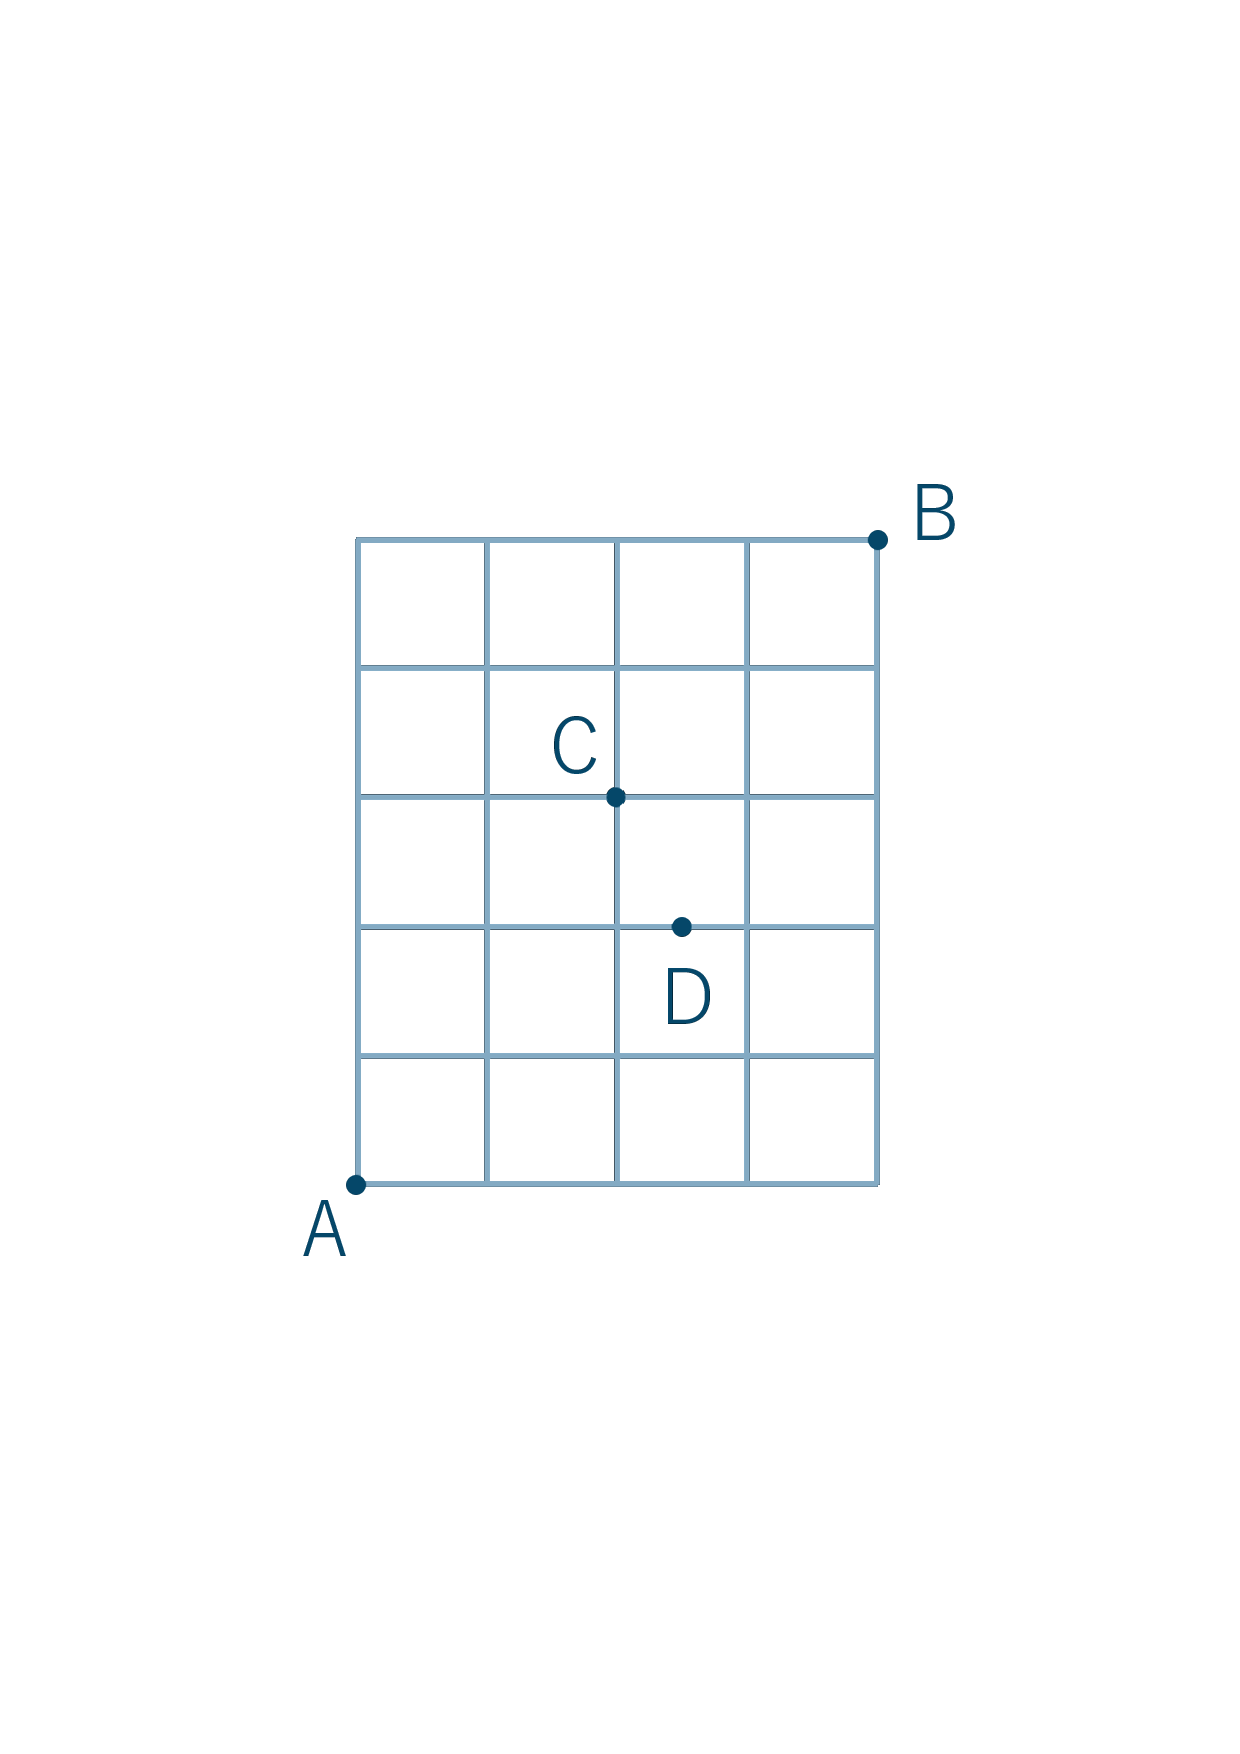
\includegraphics[width=5cm]{keiro.pdf}
  \end{wrapfigure}

  \begin{enumerate}
    \item AからBまでの最短経路
    \item AからBまでの最短経路でCを必ず通る経路
    \item AからBまでの最短経路でDを通らない経路
  \end{enumerate}
\end{itembox}
\begin{itembox}[l]{重複組合せ}
  \begin{enumerate}
    \item 6本の同種類のペンをA、B、Cの3つの袋に入れるとき、1本も入らない袋があってよいとき、分け方は何通りあるか。
    \item オレンジ、レモン、ライムがそれぞれ多数ある。これから10個をまとめてセットを作りたい。何通りのセットができるか。
  \end{enumerate}
\end{itembox}

\begin{itembox}[l]{等式を満たす整数}
  \begin{enumerate}
    \item $x+y+z=10(x,y,z:0以上の整数)$の時の組合せ
    \item $x+y+z=10(x,y,z:自然数)$の時の組合せ
  \end{enumerate}
\end{itembox}

\subsection*{確率}
\begin{itembox}[l]{確率の基本}
  コインを3枚同時に投げるとき、次の確率を求めよ。
  \begin{enumerate}
    \item 2枚だけ表である確率
    \item 表が2枚以上である確率
  \end{enumerate}
\end{itembox}
\begin{itembox}[l]{さいころの確率}
  さいころを2個同時に投げるとき、次の確率を求めよ。
  \begin{enumerate}
    \item 目の和が8となる確率
    \item 目の和が10以下となる確率
  \end{enumerate}
\end{itembox}
\begin{itembox}[l]{ボールを取り出す確率}
  赤玉5個と白玉7個が入った袋から同時に3個取り出すとき、次の確率を求めよ。
  \begin{enumerate}
    \item 白玉3個となる確率
    \item 赤玉1個、白玉2個となる確率
    \item 赤玉2個、白玉1個となる確率
  \end{enumerate}
\end{itembox}

\begin{itembox}[l]{一列に並べる確率}
  男子5人、女子4人が1列に並ぶとき、次の確率を求めよ。
  \begin{enumerate}
    \item 特定の男女が隣り合う
    \item 女子が両端にいる
    \item 男女が交互に並ぶ
  \end{enumerate}
\end{itembox}
\begin{itembox}[l]{円形に並べる確率}
  男子3人、女子3人が円卓にする座るとき、次の確率を求めよ。
  \begin{enumerate}
    \item 特定の2人が隣り合う
    \item 特定の2人が向い合う
    \item 男女が交互に座る
  \end{enumerate}
\end{itembox}
\begin{itembox}[l]{和事象と排反事象}
  1~50までの数字が書かれたカードから、1枚取り出すとき、次の確率を求めよ。
  \begin{enumerate}
    \item 2の倍数または一の位が3である2桁の数
    \item 2の倍数または3の倍数
  \end{enumerate}
\end{itembox}
\begin{itembox}[l]{余事象の確率}
  \begin{enumerate}
    \item 赤玉5個と白玉7個が入った袋から同時に3個取り出すとき、少なくとも赤玉1個を取り出す確率を求めよ。
    \item さいころを2個同時に投げるとき、目の和が3の倍数でない確率を求めよ。
  \end{enumerate}
\end{itembox}
\begin{itembox}[l]{独立試行の確率}
  Aの袋には赤玉3個と白玉2個が、Bの袋には赤玉2個と白玉4個が入っている。Aからは1個、Bからは2個の玉を取り出すとき、取り出した玉の色がすべて赤となる確率を求めよ。
\end{itembox}
\begin{itembox}[l]{反復試行の確率(コイン)}
  1枚のコインを5回連続して投げるとき、次の確率を求めよ。
  \begin{enumerate}
    \item 表がちょうど4回出る
    \item 表がちょうど3回出る
  \end{enumerate}
\end{itembox}
\begin{itembox}[l]{反復試行の確率(さいころ)}
  1個のさいころを5回連続して投げるとき、次の確率を求めよ。
  \begin{enumerate}
    \item 3の倍数の目が2回だけ出る
    \item 3の倍数の目が3回だけ出る
    \item 少なくとも1回3の倍数の目が出る
  \end{enumerate}
\end{itembox}

\begin{itembox}[l]{勝先取の確率}
  AとBが試合をし、先に3勝した方が優勝とする。Aが勝つ確率が$\frac{3}{4}$のとき、Aが優勝する確率を求めよ。
\end{itembox}

\begin{itembox}[l]{点が動く確率}
  数直線上に点Pが原点にあり、さいころを投げて5以上の目が出ると正の方向に2進み、それ以外が出ると負の方向に1進む。さいころを3回投げたとき点Pが次の位置にある確率を求めよ。
  \begin{enumerate}
    \item 原点の位置にある
    \item 座標3の位置にある
  \end{enumerate}
\end{itembox}
\begin{itembox}[l]{条件付き確率}
  ある学校で数学が好きな生徒は40\%で、英語が好きな生徒は60\%で、両方好きな生徒は30\%である。次の確率を求めよ。
  \begin{enumerate}
    \item ある生徒が数学を好きとわかっていて、その生徒が英語も好きな確率
    \item ある生徒が英語を好きとわかっていて、その生徒が数学も好きな確率
  \end{enumerate}
\end{itembox}




\begin{itembox}[l]{確率の乗法定理}
  10本中当たりが3本入ったくじがある。このくじをAが1本引き、引いたくじを元に戻さずに続けてBが引いた。このとき、AとBのそれぞれが当たる確率を求めよ。
\end{itembox}

\newpage
\subsection*{図形}
\subsubsection*{チェバの定理}

\subsubsection*{メネラウスの定理}

\subsubsection*{円と接戦の関係}
\subsubsection*{方べきの定理}
\end{document}